\section{Data and Monte Carlo Samples \label{sec:datasamples}}
This section lists the data samples and triggers that were used for the
analysis. The hadronic and W $\rightarrow$ $\mu$ $\nu$ samples are
based on the following datasets:\\
\verb!/HT/Run2011A-May10ReReco-v1/AOD! \\
\verb!/HT/Run2011A-PromptReco-v4/AOD!

For the photon control sample, the following datasets are used:\\
\verb!/Photon/Run2011A-May10ReReco-v1/AOD! \\
\verb!/Photon/Run2011A-PromptReco-v4/AOD!

The sum of data from these samples corresponds to an integrated
luminosity 1.1~fb$^{-1}$, as certified in the official JSON from 
5$^{th}$~July 2011\fixme{ADD DATE}.

The signal and background Monte Carlo samples for this analysis are
taken from a mixture of Fall10 and Spring11 simulation production for
physics at 7\TeV \\
\verb!/QCD_Pt_*_TuneZ2_7TeV_pythia6/Spring11-PU_S1_START311_V1G1-v1/AODSIM!\\
\verb!/QCD_TuneD6T_HT-*_7TeV-madgraph/Spring11-PU_S1_START311_V1G1-v1/AODSIM!\\
\verb!/TTJets_TuneZ2_7TeV-madgraph-tauola/Spring11-PU_S1_START311_V1G1-v1/AODSIM!\\
\verb!/TToBLNu_TuneZ2_*-channel_7TeV-madgraph/Spring11-PU_S1_START311_V1G1-v1/AODSIM!\\
\verb!/WJetsToLNu_TuneZ2_7TeV-madgraph-tauola/Spring11-PU_S1_START311_V1G1-v1/AODSIM!\\
\verb!/ZinvisibleJets_7TeV-madgraph/Spring11-PU_S1_START311_V1G1-v1/GEN-SIM-RECO!\\
\verb!/GJets_TuneD6T_HT-40To100_7TeV-madgraph/Spring11-PU_S1_START311_V1G1-v1/AODSIM!\\
\verb!/LM*_SUSY_sftsht_7TeV-pythia6/Spring11-PU_S1_START311_V1G1-v1/AODSIM!

\section{Triggers} % (fold)
\label{sub:triggers}

The trigger strategy has changed from that of the 2010
analysis~\cite{RA1Paper}, where a pure \HT trigger was used to collect
both the signal and the control samples.  With the increase in
instantaneous luminosity seen in 2011, the \HT thresholds of these
triggers are too high for the analysis.  In contrast to 2010, the High
Level Trigger has moved to using energy corrected jets to calculate
\HT which results in a much steeper trigger efficiency curve as a
function of \HT.  To ensure that the trigger is fully efficient with
respect to the final event selection, the offline \HT bin edges have
been shifted up by 25\GeV with respect to the online values. The
analysis therefore uses the following \HT binning: 275, 325, 375, 475,
575, 675, 775, and $>$ 875 \gev.

To select candidate events with jets + missing transverse energy,
cross-object triggers between \HT and $\mht = |\vec{\mht}| =
|\sum_{i=1}^{n} \vec{\pt}^{\rm jet_i}|$ are used.  Due to evolving
trigger thresholds on the \mht part of the trigger over the period of
data collection, a small inefficiency of $0.99^{+0.01}_{-0.02} $ is
encountered in the lowest \HT = 275 \gev bin and corrected for.  In
the \HT = 325 \gev (375 \gev) bins, the trigger is fully efficient
with a statistical uncertainty of 3.4\% (3.2\%). The trigger paths
used to collect the hadronic sample are: \verb!HLT_HT260_MHT60_v*!,
\verb!HLT_HT250_MHT50_v*,!, \verb!HLT_HT250_MHT60_v*!,
\verb!HLT_HT250_MHT70_v*!, \verb!HLT_HT250_MHT80_v*! and
\verb!HLT_HT250_MHT90_v*!.

A suite of prescaled \HT triggers is used to select events which stem
mainly in QCD multi-jet production.  A photon control sample to
constrain the background from \znunu\ events is selected with a single
object photon trigger. The triggers used to collect the photon control
sample are \verb!HLT_Photon75_CaloIdVL!,
\verb!HLT_Photon75_CaloIdVL_IsoL!, \verb!HLT_Photon90_CaloIdVL! and
\verb!HLT_Photon90_CaloIdVL_IsoL!.

\begin{figure}[h!]
    \centering
     \subfigure[]{
          \label{fig:figures_HT_all}
          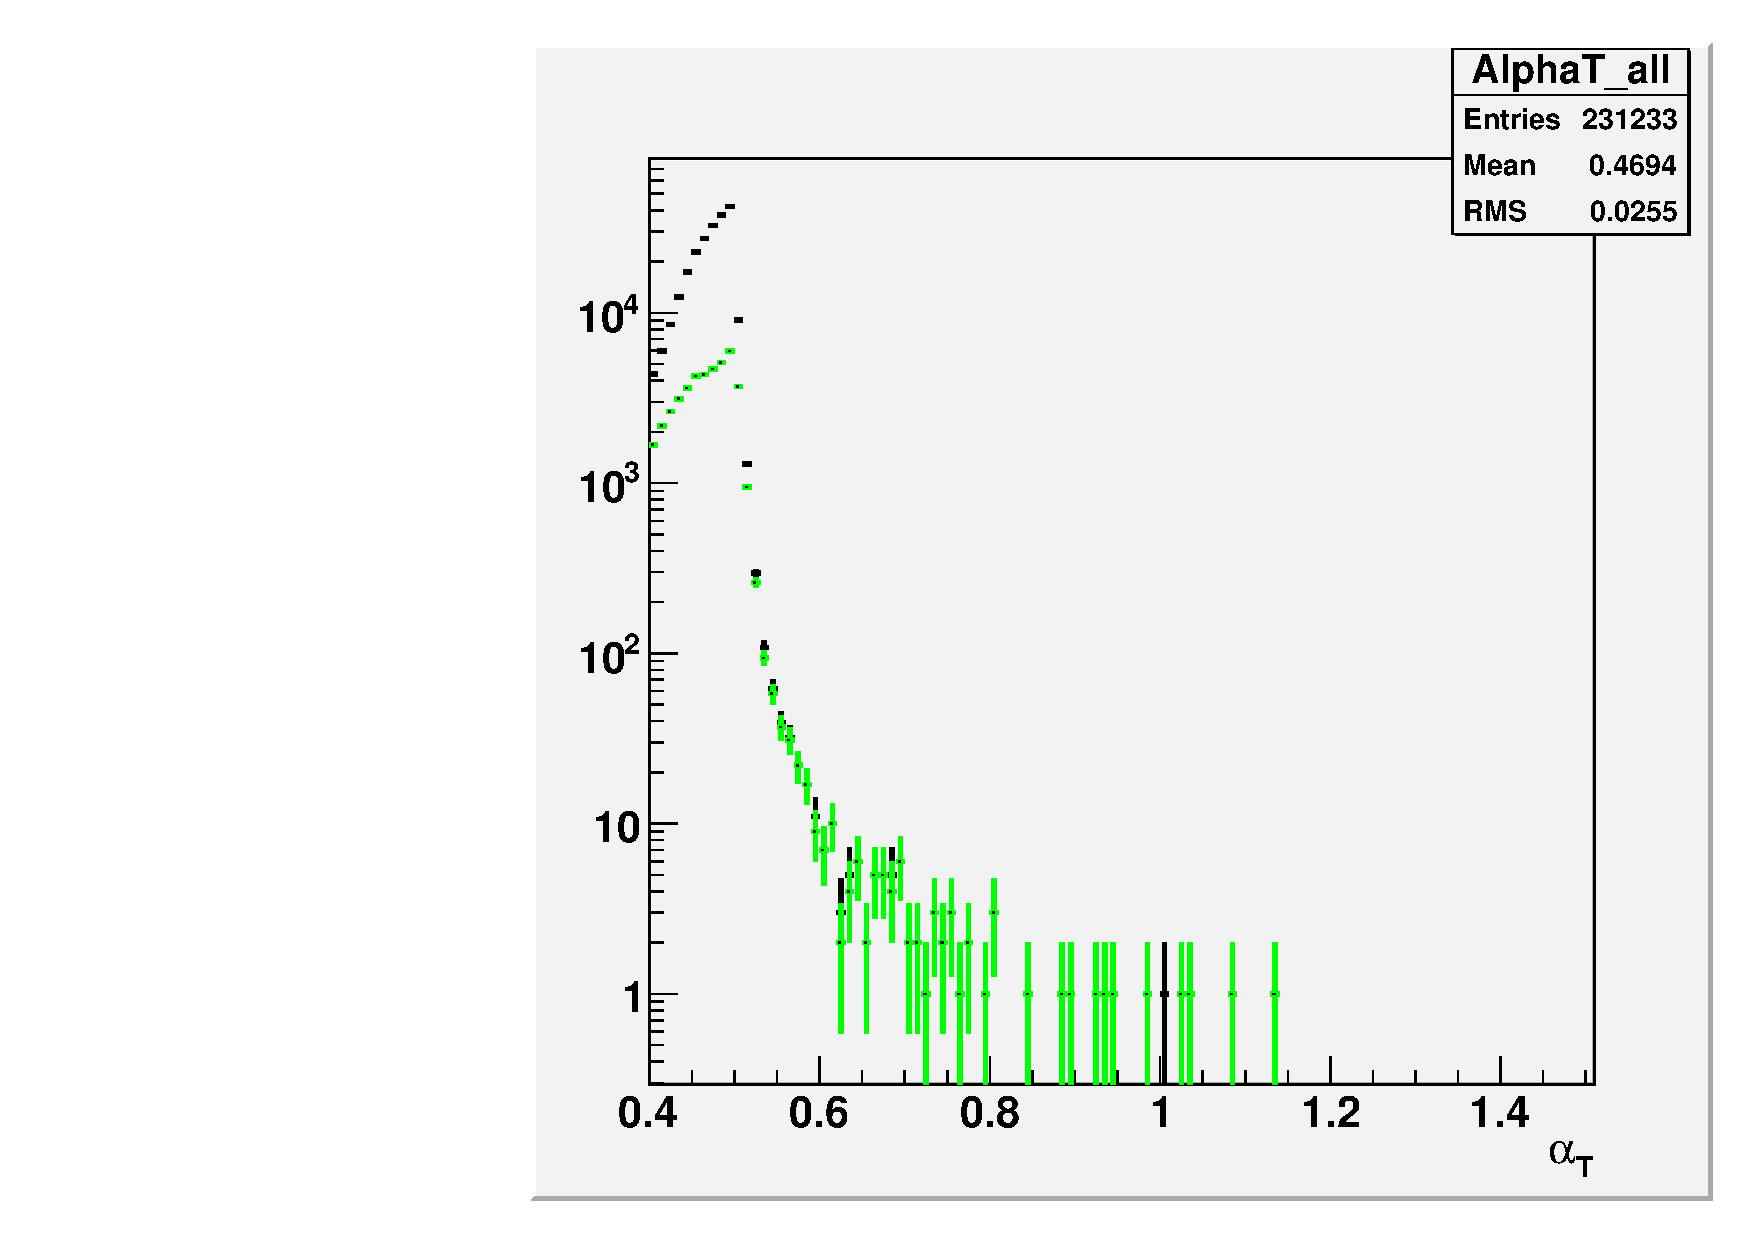
\includegraphics[width=0.46\textwidth]{figures/Trigger/MHT36AlphaT_allRAW.pdf}
     }
    \subfigure[]{
          \label{fig:figures_JetMultiplicity_all}
          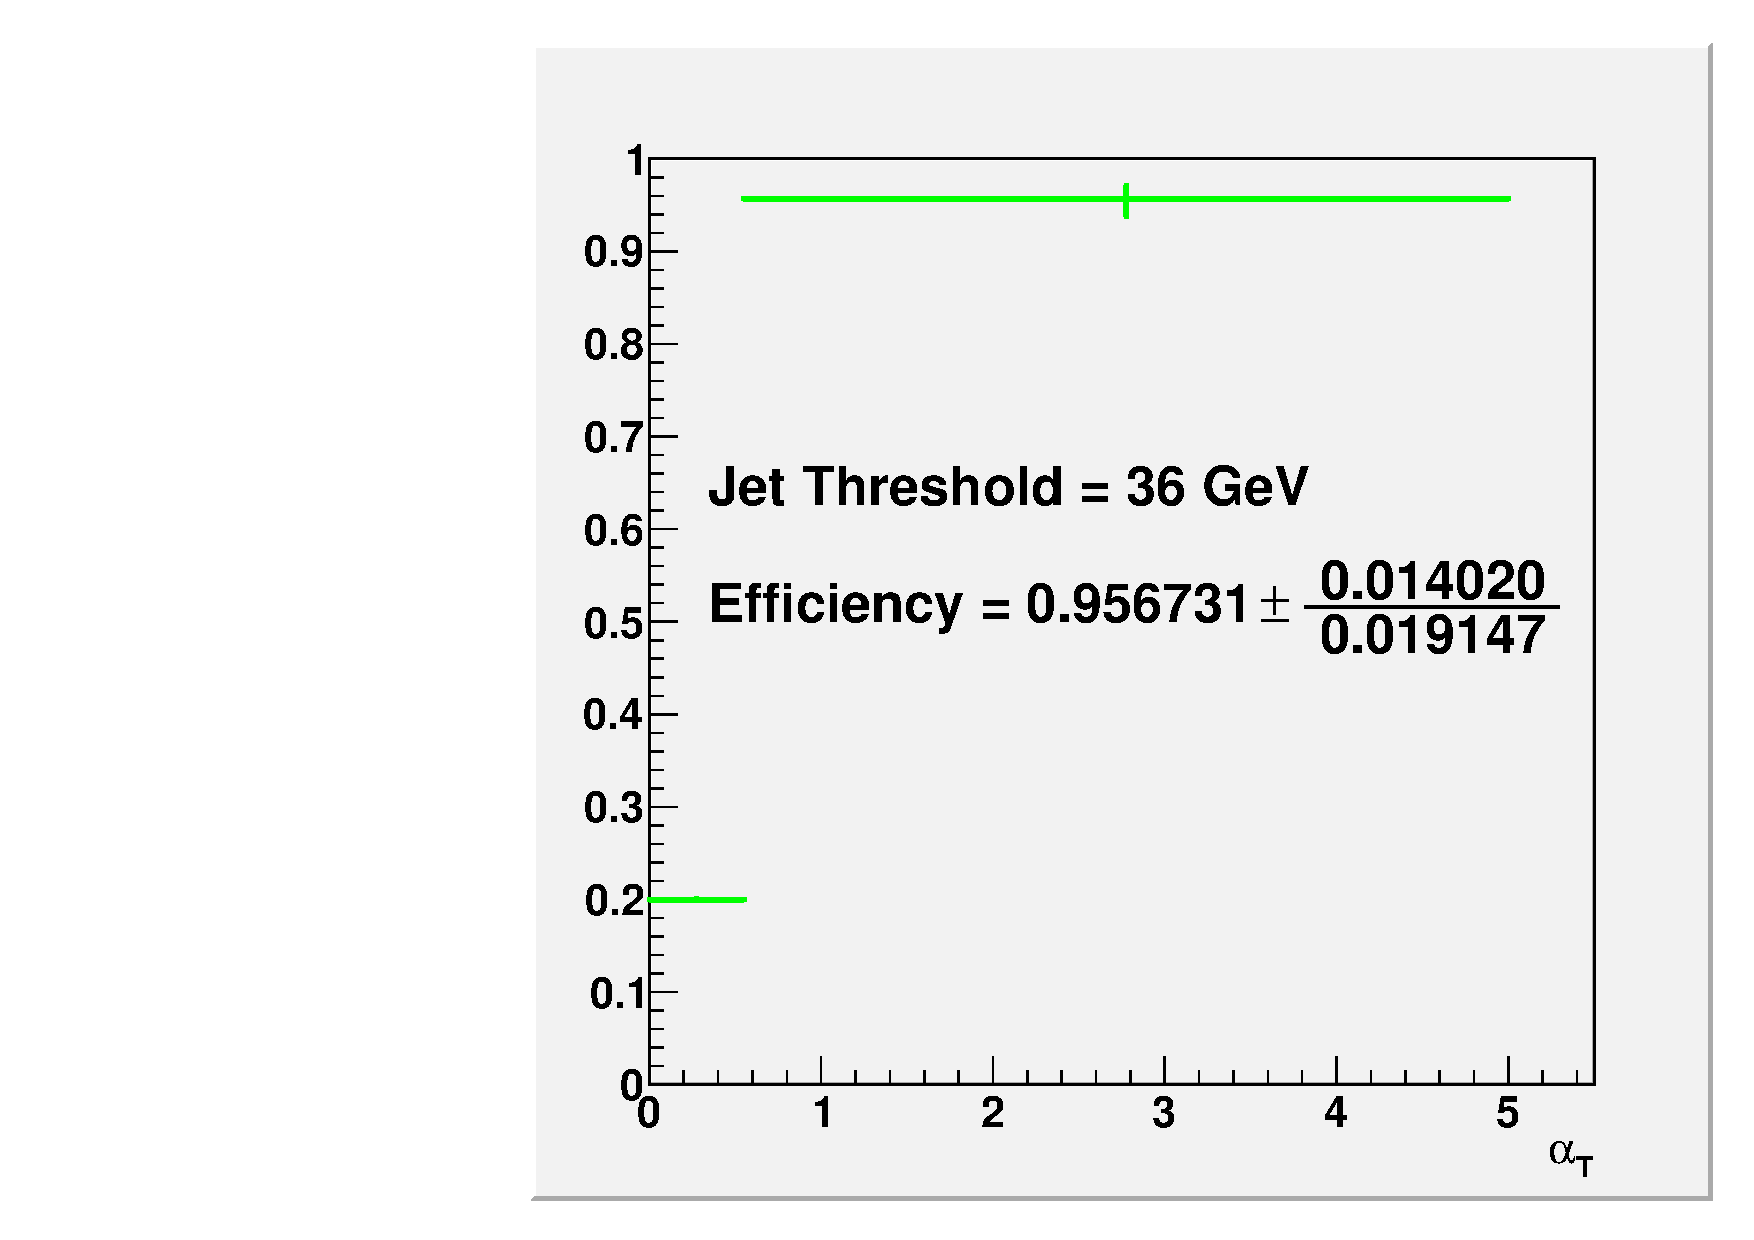
\includegraphics[width=0.46\textwidth]{figures/Trigger/MHT36AlphaT_allCumlative.pdf}
     }
     \caption{Efficiency of the HT, MHT cross trigger in the lowest
       scaled bin, Jet \PT threshold $\geq $ 36.$\dot{6}$ GeV.  (a)
       Comparison of the \alt distributions from two sets of triggers,
       the black points come from a Muon based trigger and act as the
       denominator for the turn on curve, where as the green points
       come from the logical and of the HT, MHT cross trigger and the
       Muon trigger. (b) Efficiency of the HT, MHT cross trigger, in
       the \alt plane.}
\end{figure}

\begin{figure}[h!]
    \centering
     \subfigure[]{
          \label{fig:figures_HT_all}
          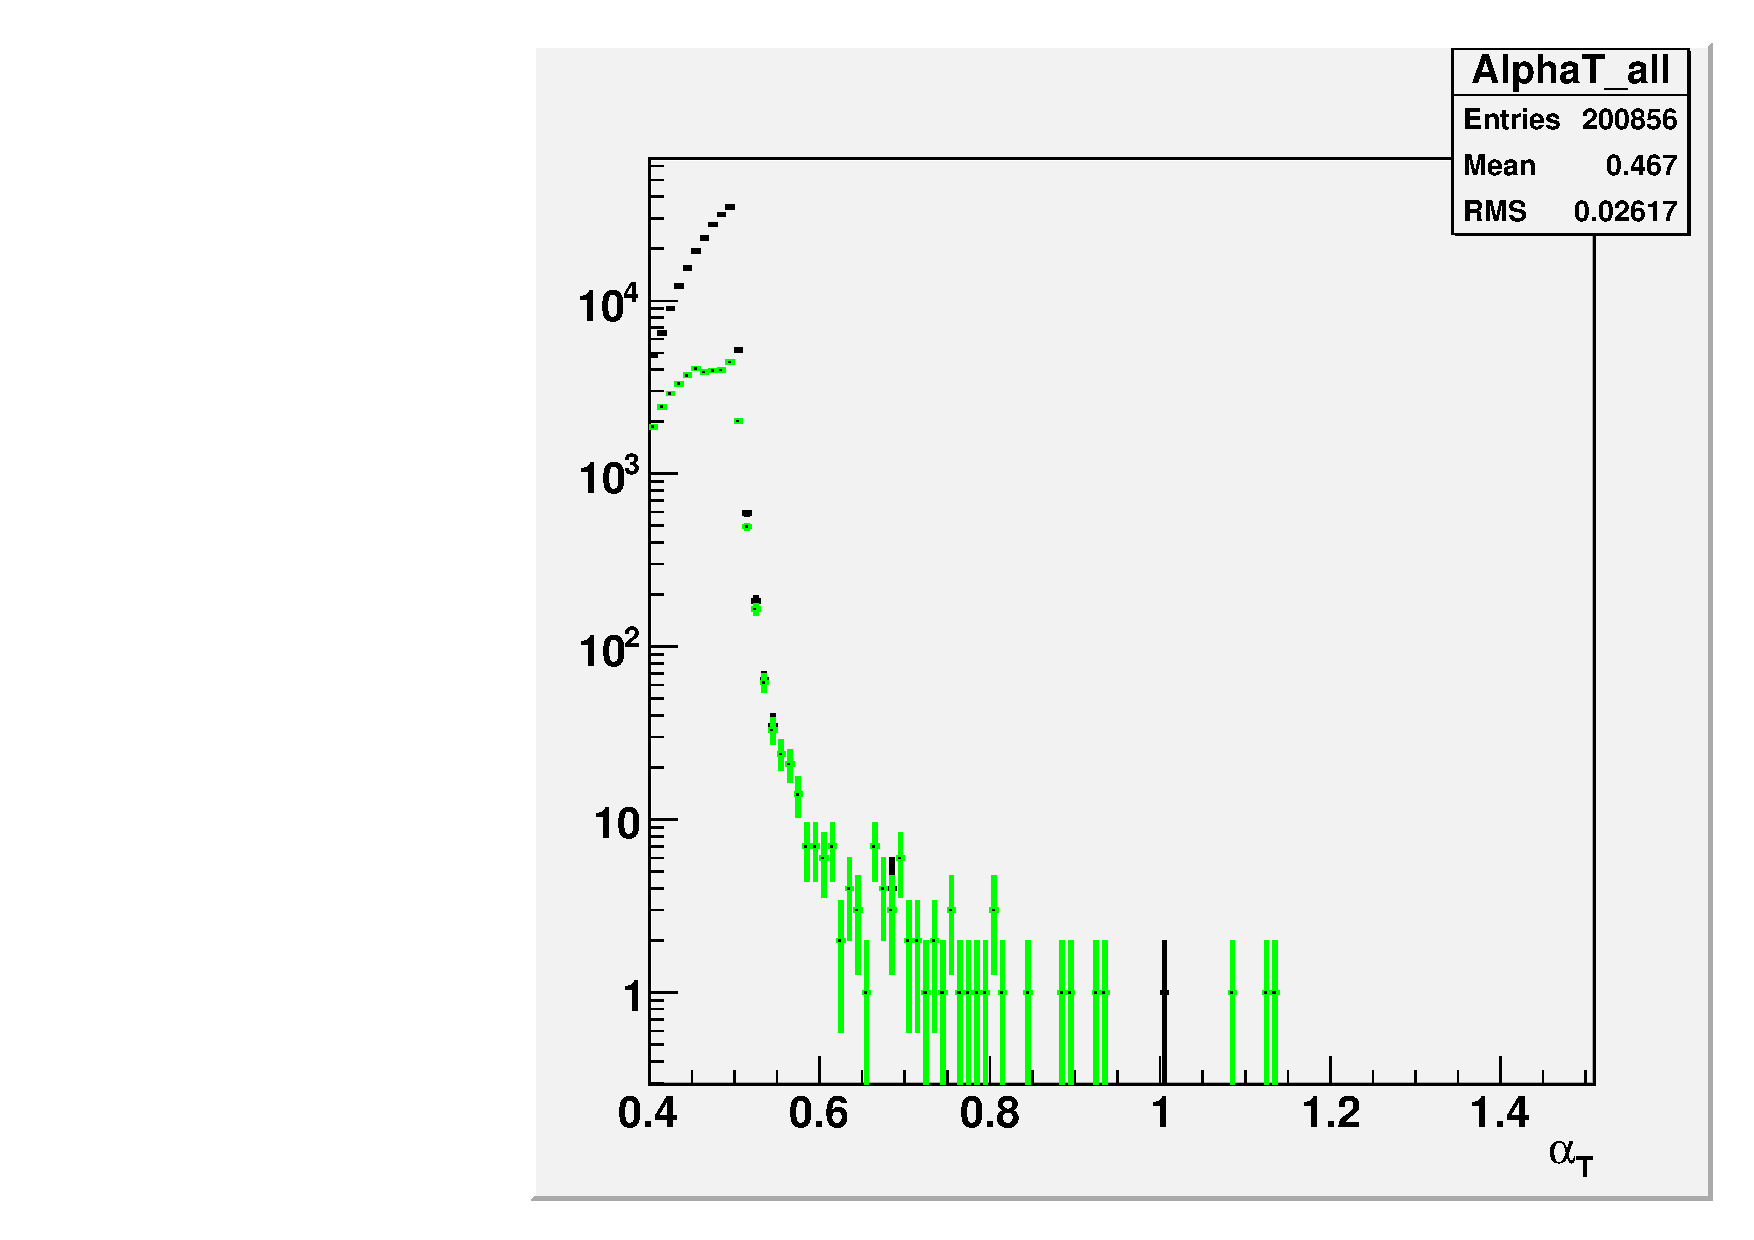
\includegraphics[width=0.46\textwidth]{figures/Trigger/MHT43AlphaT_allRAW.pdf}
     }
    \subfigure[]{
          \label{fig:figures_JetMultiplicity_all}
          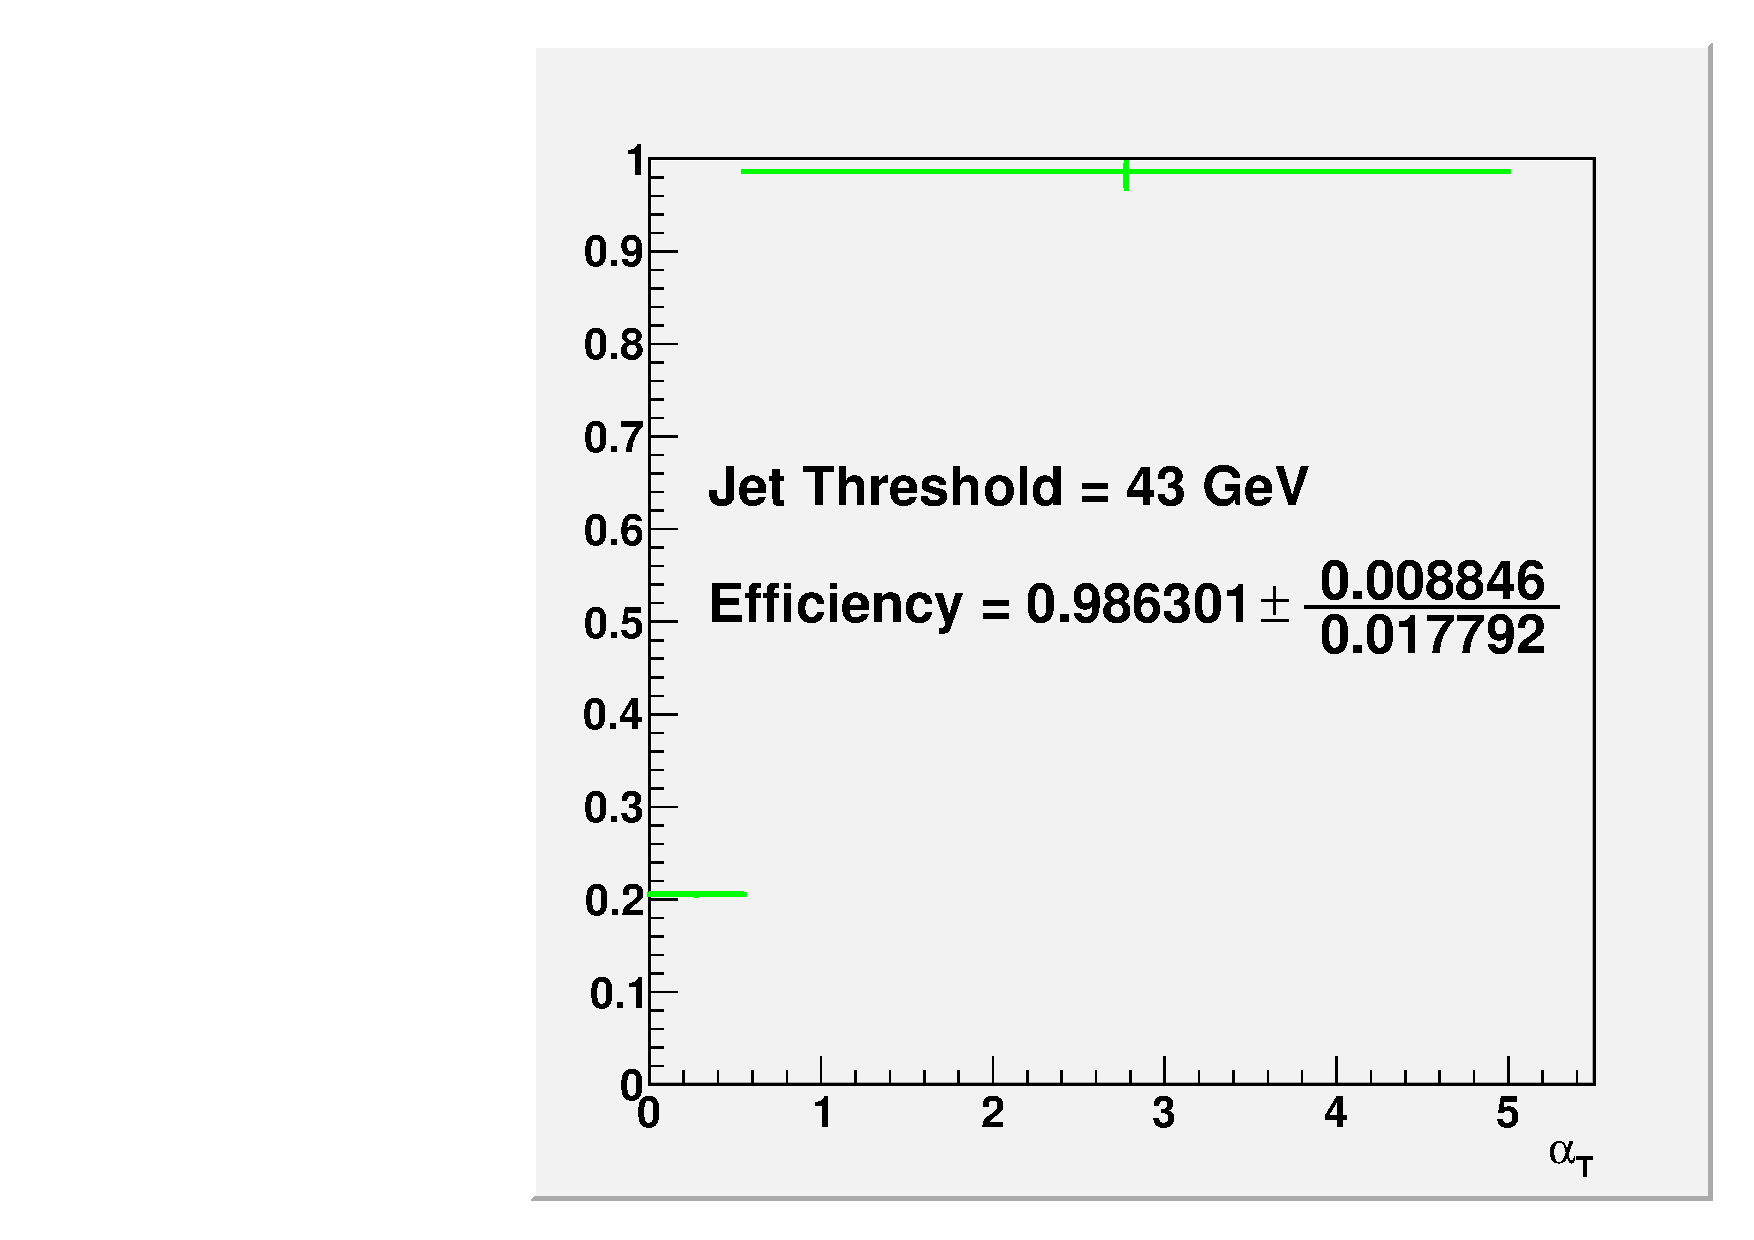
\includegraphics[width=0.46\textwidth]{figures/Trigger/MHT43AlphaT_allCumlative.pdf}
     }
     \caption{Efficiency of the HT, MHT cross trigger in the lowest
       scaled bin, Jet \PT threshold $\geq $ 43.$\dot{3}$ GeV.  (a)
       Comparison of the \alt distributions from two sets of triggers,
       the black points come from a Muon based trigger and act as the
       denominator for the turn on curve, where as the green points
       come from the logical and of the HT, MHT cross trigger and the
       Muon trigger. (b) Efficiency of the HT, MHT cross trigger, in
       the \alt plane.}
\end{figure}


\begin{figure}[h!]
    \centering
     \subfigure[]{
          \label{fig:figures_HT_all}
          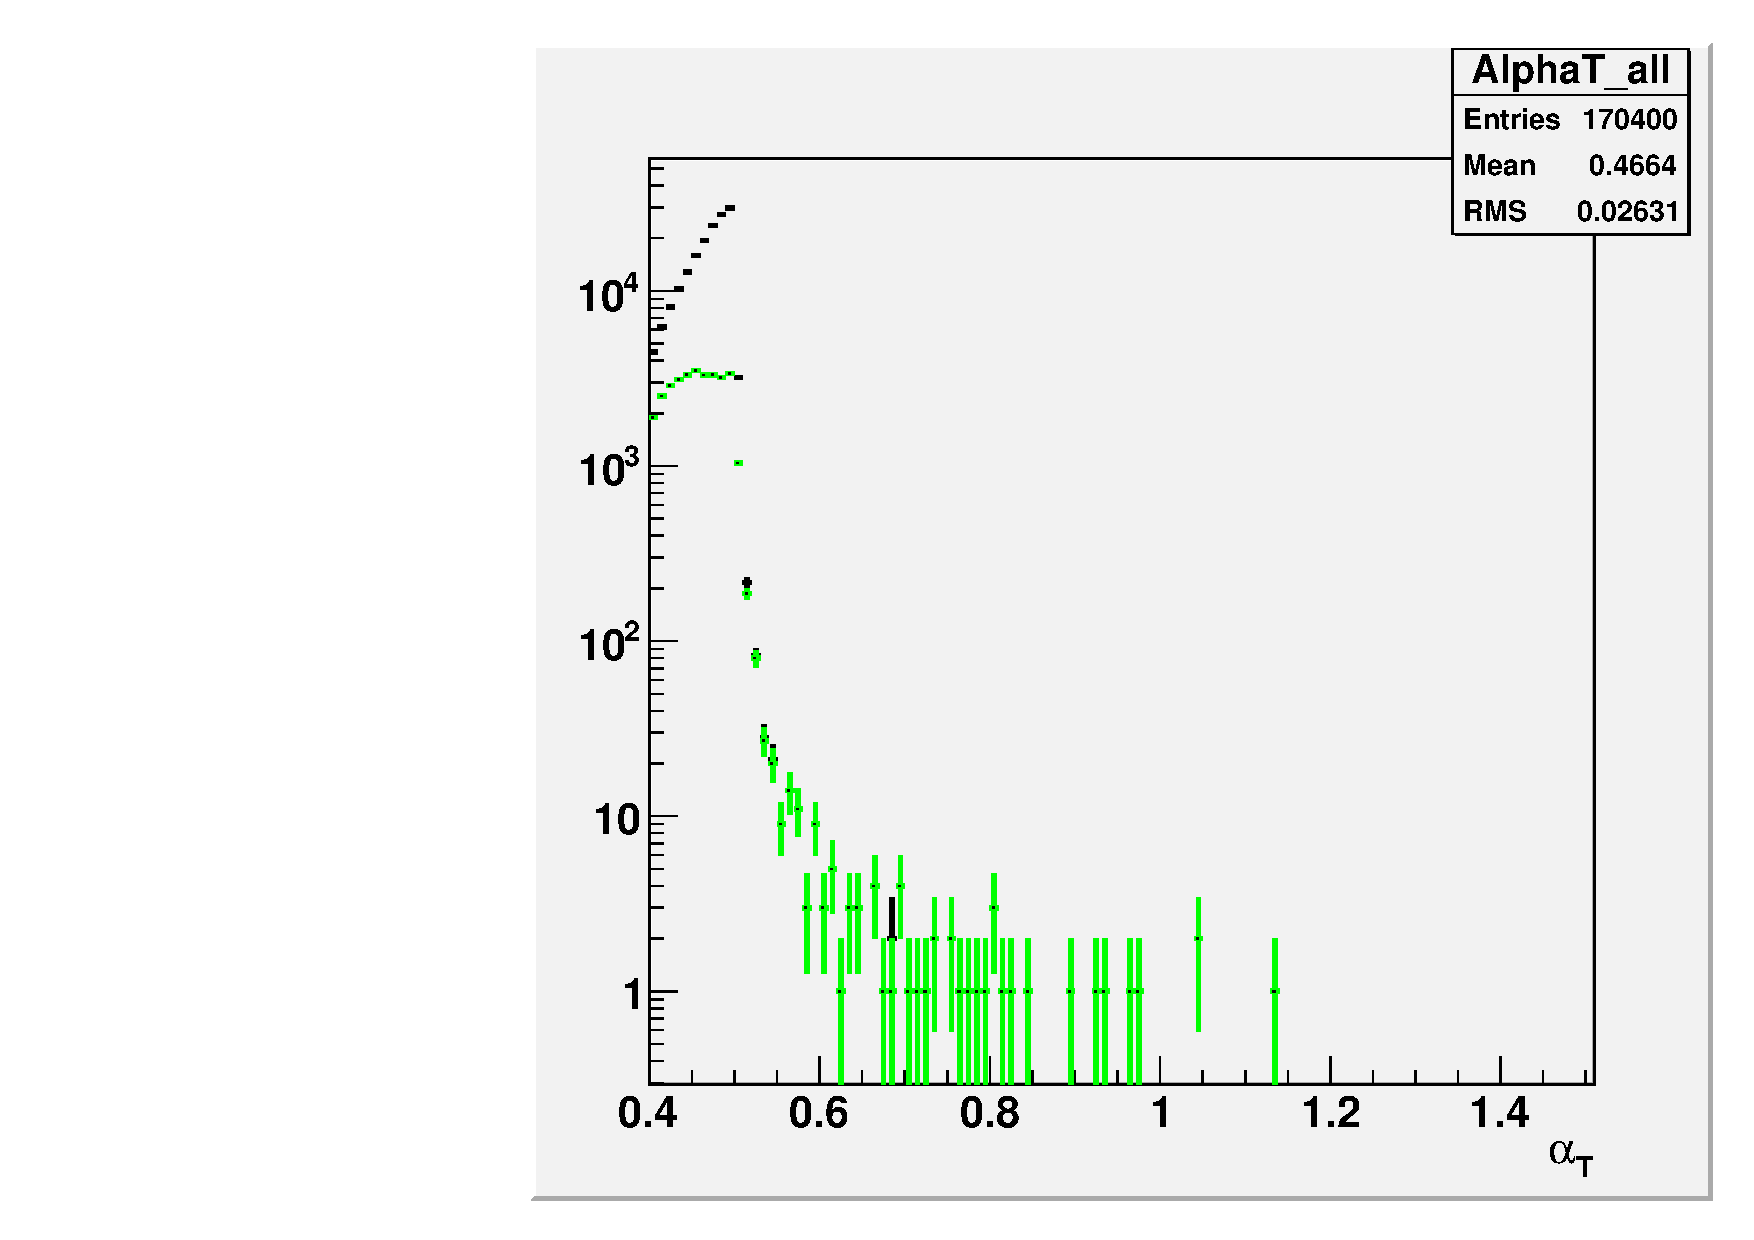
\includegraphics[width=0.46\textwidth]{figures/Trigger/MHT50AlphaT_allRAW.pdf}
     }
    \subfigure[]{
          \label{fig:figures_JetMultiplicity_all}
          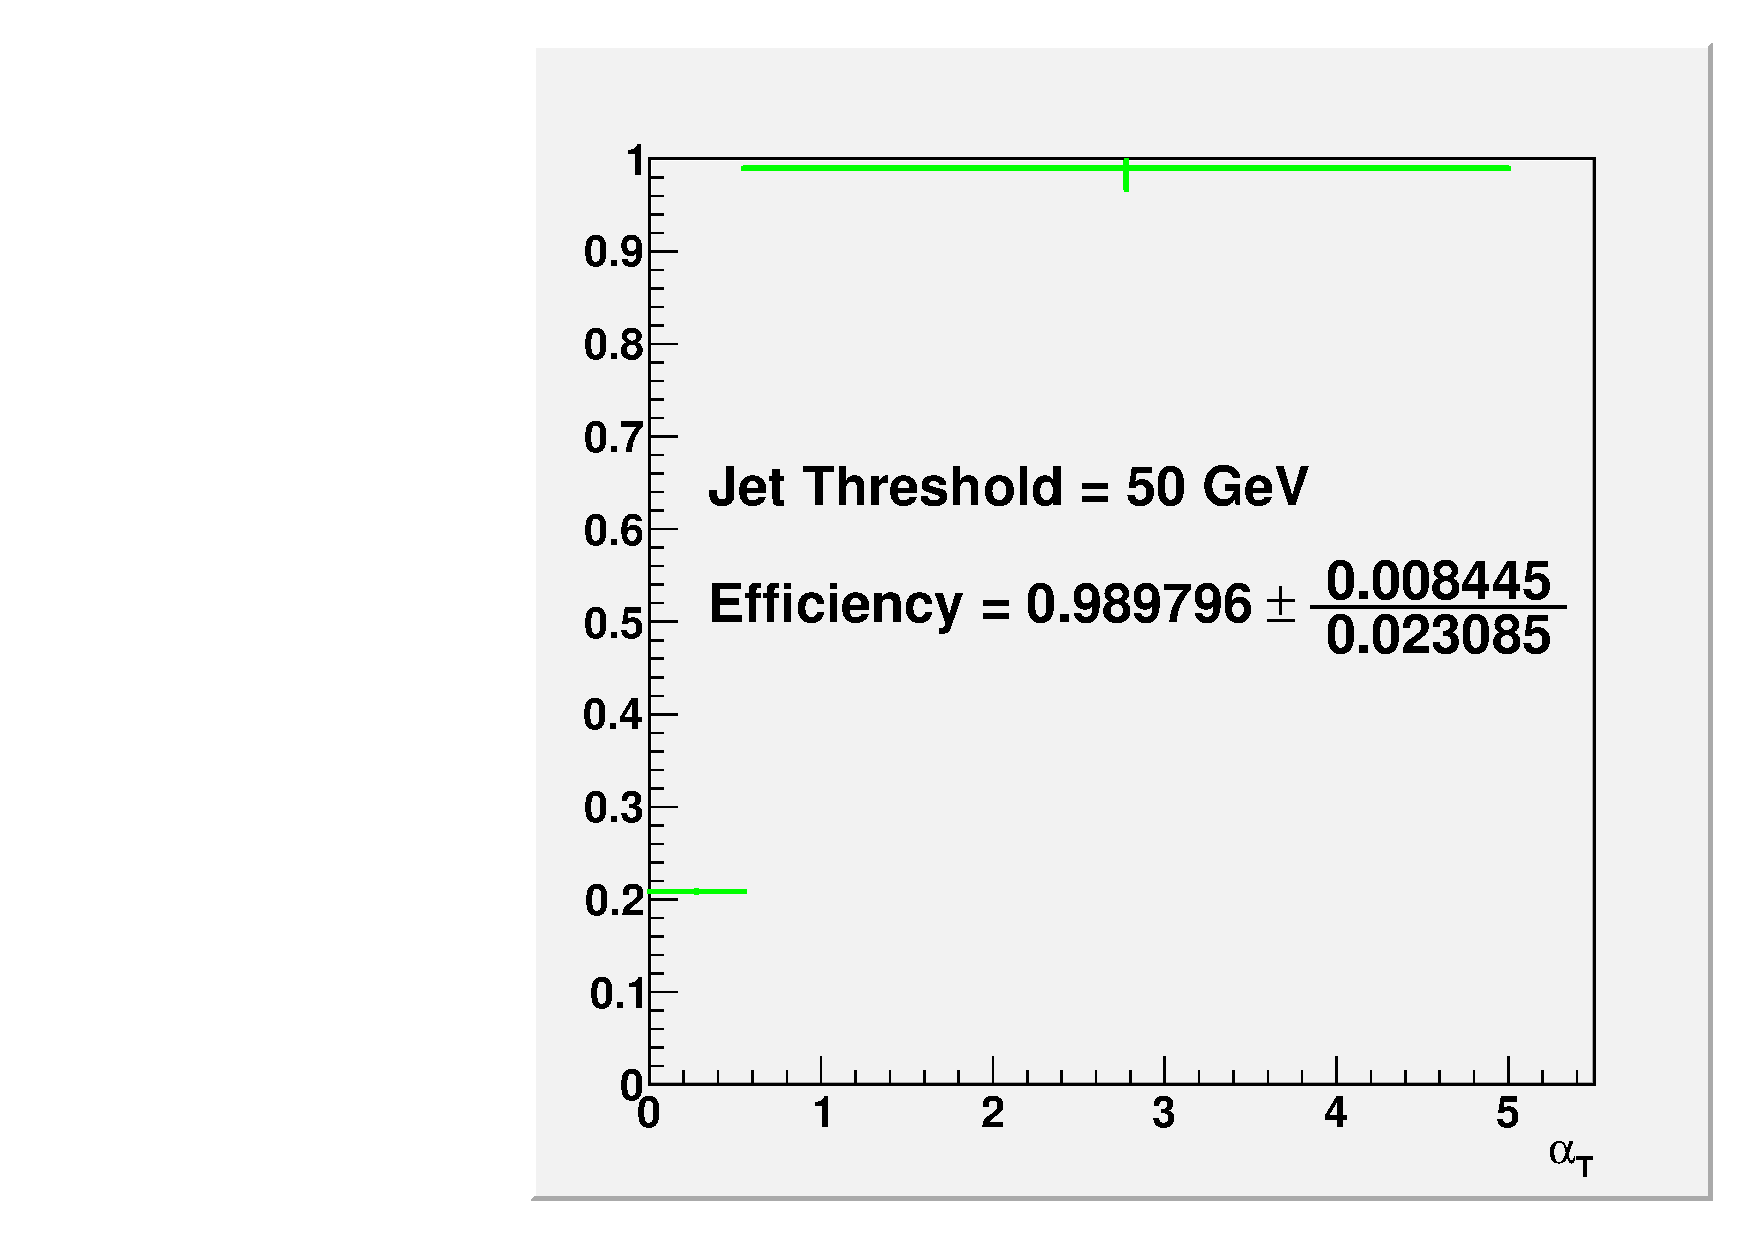
\includegraphics[width=0.46\textwidth]{figures/Trigger/MHT50AlphaT_allCumlative.pdf}
     }
     \caption{Efficiency of the HT, MHT cross trigger in the lowest
       scaled bin, Jet \PT threshold $\geq $ 50.0 GeV.  (a) Comparison
       of the \alt distributions from two sets of triggers, the black
       points come from a Muon based trigger and act as the
       denominator for the turn on curve, where as the green points
       come from the logical and of the HT, MHT cross trigger and the
       Muon trigger. (b) Efficiency of the HT, MHT cross trigger, in
       the \alt plane.}
\end{figure}
